% Fig. 2: Schema of the per-stay heterogeneous patient-concept graph (vector, Times 8 pt).
\documentclass[10pt,border=1pt]{standalone}
\usepackage{mathptmx}
\usepackage{tikz}
\usetikzlibrary{arrows.meta,positioning,calc}
\begin{document}
\footnotesize
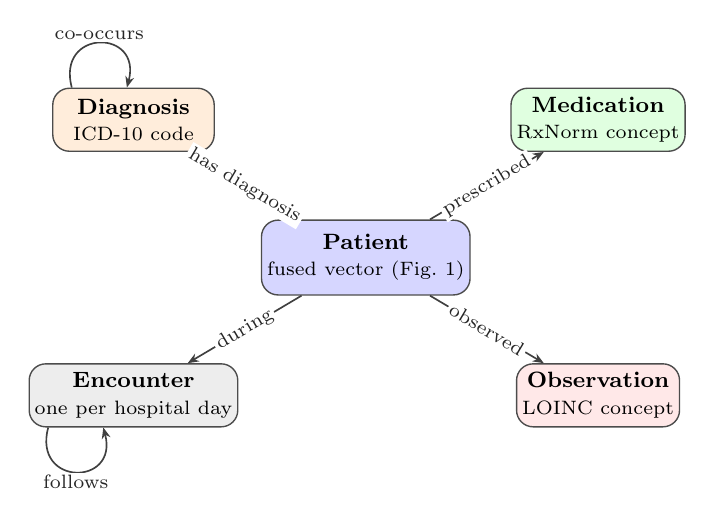
\begin{tikzpicture}[
  font=\footnotesize,
  >={Stealth[length=4pt,width=3.2pt]},
  nd/.style={draw=black!70, line width=0.5pt, rounded corners=6pt, align=center,
             minimum width=2.05cm, minimum height=0.80cm, inner sep=2pt},
  rel/.style={->, draw=black!75, line width=0.6pt},
  rl/.style={font=\scriptsize, fill=white, inner sep=1pt, text=black!85}
]
\node[nd, fill=blue!16, minimum width=2.2cm, minimum height=0.95cm] (p) at (0,0)
  {\textbf{Patient}\\ \scriptsize fused vector (Fig.~1)};
\node[nd, fill=orange!14] (d) at (-2.95, 1.75) {\textbf{Diagnosis}\\ \scriptsize ICD-10 code};
\node[nd, fill=green!12]  (m) at ( 2.95, 1.75) {\textbf{Medication}\\ \scriptsize RxNorm concept};
\node[nd, fill=red!9]     (o) at ( 2.95,-1.75) {\textbf{Observation}\\ \scriptsize LOINC concept};
\node[nd, fill=black!7]   (e) at (-2.95,-1.75) {\textbf{Encounter}\\ \scriptsize one per hospital day};

\draw[rel] (p) -- node[rl, sloped] {has diagnosis} (d);
\draw[rel] (p) -- node[rl, sloped] {prescribed} (m);
\draw[rel] (p) -- node[rl, sloped] {observed} (o);
\draw[rel] (p) -- node[rl, sloped] {during} (e);

% self relations
\draw[rel] (d.north west) ++(0.25,0) .. controls +(-0.2,0.75) and +(0.2,0.75) .. ([xshift=0.95cm]d.north west)
  node[pos=0.5, above, rl] {co-occurs};
\draw[rel] (e.south west) ++(0.25,0) .. controls +(-0.2,-0.75) and +(0.2,-0.75) .. ([xshift=0.95cm]e.south west)
  node[pos=0.5, below, rl] {follows};
\end{tikzpicture}
\end{document}
